\documentclass[10pt,a4paper]{article}
\usepackage{schedule_style}
\usepackage{color}
\definecolor{light-gray}{gray}{0.95}
\pagecolor{light-gray}

\fboxsep=0mm%padding thickness
\fboxrule=1pt%border thickness

\lhead{Hotcit::Tasks}
\rhead{\today}
\begin{document}
%%%
\begin{quote}

\tdos
\tdo revisit server
\tdo set up a build script for server deployment from command line
\tdo try to run existing unit tests
\tdo add to repository, a client skeleton
\tod write a preliminary task list
\tdo checkout \\
\verb|http://www.brettspielwelt.de/Hilfe/Anleitungen/OhneFurchtUndAdel|

\vspace{1em}
\tdo sketch client visual layout
\tdo set up a mock up backed game with 1 player

\vspace{1em}
\tdo display player's starting hand
\tdo display player's starting gold
\tdo display player's districts (start with 3)
\tdo display player's public points (5)
\tdo display player's personality (King)
\tdo display turn number
\tdo display whose turn it is
\tdo display available actions

\vspace{1em}
\tdo render and allow player to build a district
\tdo render and allow player to draw gold
\tdo render and allow  player to use action
\tdo render and allow  player to draw a card
\tdo render and allow  player to end turn

\vspace{1em}
\tdo display three other players ...
\tdoe

\vspace{2em}\hspace{1em}{\fbox{\centering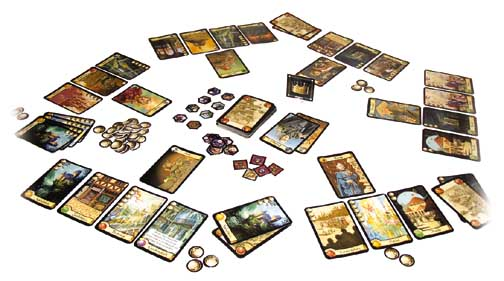
\includegraphics[scale=0.5]{citadels.jpg}}}
\end{quote}
%%%
\end{document}